% !TEX root = ../Thesis.tex

\chapter{Introduction}\
\label{ch:introduction}



\section{Motivation and Literature Review}\
\label{ch:motivation}
%(Context and justification, why is this work important?)\\

Buildings are at the heart of society, and have a large impact on global health, economics and the environment. Europeans alone spend on average 90\% of their time in buildings \cite{Staniaszek2014BPIE} whether it be for work, rest or the multitude of activities that exists in modern society...\\

  \begin{figure}[ht] %h can be omitted for better page layout
    \begin{center}
      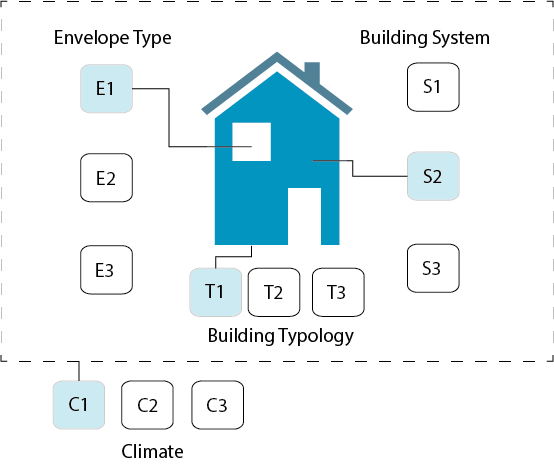
\includegraphics[width=\textwidth, trim= 0cm 0cm 0cm 0cm,clip]{envelope_system_comparison.png}
      \caption{Figure Example}
      \label{fig: comparison}
    \end{center} 
  \end{figure}

 
\section{Problem Statement}\
%What is the problem that you are trying to solve?
A big problem is on the horizon


\section{Objectives of Research}\
%(What do you want to achieve, more in general terms? Bullet point list)\\

Based on the problem statement, the objectives are to

\begin{itemize}
	\item Objective 1
	\item Objective 2
\end{itemize}


\section{Thesis Outline}\
%Breakdown of your thesis (Not always necessary)


